\documentclass[english,floatsintext,man]{apa6}

\usepackage{amssymb,amsmath}
\usepackage{ifxetex,ifluatex}
\usepackage{fixltx2e} % provides \textsubscript
\ifnum 0\ifxetex 1\fi\ifluatex 1\fi=0 % if pdftex
  \usepackage[T1]{fontenc}
  \usepackage[utf8]{inputenc}
\else % if luatex or xelatex
  \ifxetex
    \usepackage{mathspec}
    \usepackage{xltxtra,xunicode}
  \else
    \usepackage{fontspec}
  \fi
  \defaultfontfeatures{Mapping=tex-text,Scale=MatchLowercase}
  \newcommand{\euro}{€}
\fi
% use upquote if available, for straight quotes in verbatim environments
\IfFileExists{upquote.sty}{\usepackage{upquote}}{}
% use microtype if available
\IfFileExists{microtype.sty}{\usepackage{microtype}}{}

% Table formatting
\usepackage{longtable,booktabs}
\usepackage[counterclockwise]{rotating}   % Landscape page setup for large tables
\usepackage{multirow}		% Table styling
\usepackage{tabularx}		% Control Column width
\usepackage[flushleft]{threeparttable}	% Allows for three part tables with a specified notes section
\usepackage{threeparttablex}            % Lets threeparttable work with longtable
\usepackage{longtable}              % Allows tables to break across pages

  \usepackage{graphicx}
  \makeatletter
  \def\maxwidth{\ifdim\Gin@nat@width>\linewidth\linewidth\else\Gin@nat@width\fi}
  \def\maxheight{\ifdim\Gin@nat@height>\textheight\textheight\else\Gin@nat@height\fi}
  \makeatother
  % Scale images if necessary, so that they will not overflow the page
  % margins by default, and it is still possible to overwrite the defaults
  % using explicit options in \includegraphics[width, height, ...]{}
  \setkeys{Gin}{width=\maxwidth,height=\maxheight,keepaspectratio}
\ifxetex
  \usepackage[setpagesize=false, % page size defined by xetex
              unicode=false, % unicode breaks when used with xetex
              xetex]{hyperref}
\else
  \usepackage[unicode=true]{hyperref}
\fi
\hypersetup{breaklinks=true,
            pdfauthor={},
            pdftitle={How to do Effective and Sucessful Bank Telemarketing},
            colorlinks=true,
            citecolor=blue,
            urlcolor=blue,
            linkcolor=black,
            pdfborder={0 0 0}}
\urlstyle{same}  % don't use monospace font for urls

\setlength{\parindent}{0pt}
%\setlength{\parskip}{0pt plus 0pt minus 0pt}

\setlength{\emergencystretch}{3em}  % prevent overfull lines

\setcounter{secnumdepth}{0}
\ifxetex
  \usepackage{polyglossia}
  \setmainlanguage{}
\else
  \usepackage[english]{babel}
\fi

% Manuscript styling
\captionsetup{font=singlespacing,justification=justified}
\usepackage{csquotes}

 % Line numbering
  \usepackage{lineno}
  \linenumbers


\usepackage{tikz} % Variable definition to generate author note

% fix for \tightlist problem in pandoc 1.14
\providecommand{\tightlist}{%
  \setlength{\itemsep}{0pt}\setlength{\parskip}{0pt}}

% Essential manuscript parts
  \title{How to do Effective and Sucessful Bank Telemarketing}

  \shorttitle{Predictive Modeling with Losgistic Regression}


  \author{
          Arindam Barman\textsuperscript{1},
          Mohamed Elmoudni\textsuperscript{1},
          Shazia Khan\textsuperscript{1},
          Kishore Prasad\textsuperscript{1}  }

  \def\affdep{{"", "", "", ""}}%
  \def\affcity{{"", "", "", ""}}%

  \affiliation{
    \vspace{0.5cm}
          \textsuperscript{1} City University of New York (CUNY)  }


%   \def\affinst{{"init", "City University of New York (CUNY)"}}%
%   \def\affstate{{"init", ""}}%
%   \def\affcntry{{"init", ""}}%

 % If no note is defined give only author information if available
    \note{
    \vspace{1cm}
    Author note

    \raggedright
    \setlength{\parindent}{0.4in}

    \newcounter{author}

%     %       %       \setcounter{author}{0}
%         %           \addtocounter{author}{1}
%         %         \expandafter\edef\csname authorid\endcsname{\theauthor}
%         Arindam Barman, \pgfmathparse{\affdep[\authorid]} \pgfmathresult, \pgfmathparse{\affinst[\authorid]} \pgfmathresult, \pgfmathparse{\affcity[\authorid]} \pgfmathresult, \pgfmathparse{\affstate[\authorid]} \pgfmathresult, \pgfmathparse{\affcntry[\authorid]} \pgfmathresult
%       %     ;
%     %       %       \setcounter{author}{0}
%         %           \addtocounter{author}{1}
%         %         \expandafter\edef\csname authorid\endcsname{\theauthor}
%         Mohamed Elmoudni, \pgfmathparse{\affdep[\authorid]} \pgfmathresult, \pgfmathparse{\affinst[\authorid]} \pgfmathresult, \pgfmathparse{\affcity[\authorid]} \pgfmathresult, \pgfmathparse{\affstate[\authorid]} \pgfmathresult, \pgfmathparse{\affcntry[\authorid]} \pgfmathresult
%       %     ;
%     %       %       \setcounter{author}{0}
%         %           \addtocounter{author}{1}
%         %         \expandafter\edef\csname authorid\endcsname{\theauthor}
%         Shazia Khan, \pgfmathparse{\affdep[\authorid]} \pgfmathresult, \pgfmathparse{\affinst[\authorid]} \pgfmathresult, \pgfmathparse{\affcity[\authorid]} \pgfmathresult, \pgfmathparse{\affstate[\authorid]} \pgfmathresult, \pgfmathparse{\affcntry[\authorid]} \pgfmathresult
%       %     ;
%     %       %       \setcounter{author}{0}
%         %           \addtocounter{author}{1}
%         %         \expandafter\edef\csname authorid\endcsname{\theauthor}
%         Kishore Prasad, \pgfmathparse{\affdep[\authorid]} \pgfmathresult, \pgfmathparse{\affinst[\authorid]} \pgfmathresult, \pgfmathparse{\affcity[\authorid]} \pgfmathresult, \pgfmathparse{\affstate[\authorid]} \pgfmathresult, \pgfmathparse{\affcntry[\authorid]} \pgfmathresult
%       %     .

                                                      }
  
  \abstract{the Title page, the Abstract page, and the references page do not count
when using APA Style \ldots{} as such, you need to have 12 pages besides
those three pages use 250 words or less to summarize your problem,
methodology, and major outcomes. Even though direct marketing is a
standard method for banks to utilize in the face of competition and
financial unstability, it has, however, been shown to exhibit poor
performance. The telemarketing calls are simply not answered or answered
and immediately disconnected. It is however welcomed by the right person
who is in need of financial relief. The aim of this exercise is to
target clients more effectively and efficiently based on the data from a
Portuguese bank telemarketing effort. We first used logistic regression
to predict the binary response variable. The outcomes\ldots{}.}
  \keywords{select a few key words (up to five) related to your
work\ldots{}.logistic regression model, linear discriminant analysis
(LDA), predictive modeling, bank telemarketing, direct marketing, Data
Mining \\

    
  }


\begin{document}

\maketitle



\section{Introduction}\label{introduction}

describe the background and motivation of your problem--

After looking at various options, we settled for this project for our
final since it met all the requirements.

\enquote{Regression analysis is one of the most commonly used
statistical techniques in social and behavioral sciences as well as in
physical sciences. Its main objective is to explore the relationship
between a dependent variable and one or more independent variables
(which are also called predictor or explanatory variables).} This is the
definition provided by www.unesco.org for Regression Analysis

The most successful direct marketing is to predict the customers that
have a higher probability to do business. Data exploration technique, is
crucial to understand customer behavior. Many banks and services are
moving to adopt the predictive technique based on the data mining to
predict the customer profile before targeting them. The prediction or
classification is the most important task in the data exploration and
model building that is usually applied to classify the group of data. In
classification, the outcome is a categorical variable and several
combinations of input variable are used to build a model and the model
that gives a better prediction with the best accuracy is chosen to
target the prospective customers.

The data set contains approximately 41188 obs. of 21 variables.

This dataset is based on \enquote{Bank Marketing} UCI dataset (please
check the description at:
\url{http://archive.ics.uci.edu/ml/datasets/Bank+Marketing}). The data
is enriched by the addition of five new social and economic
features/attributes (national wide indicators from a
\textasciitilde{}10M population country), published by the Banco de
Portugal and publicly available at:
\url{https://www.bportugal.pt/estatisticasweb}.

The binary classification goal is to predict if the client will
subscribe a bank term deposit (variable y).

This dependent variable tells whether the client will subscribe a bank
term deposit or not. This is a binary variable and as such we will be
using a Logistic Regression Model.

\section{Literature Review}\label{literature-review}

\begin{verbatim}
There have been a few papers that have discussed this requirement.  A common thread across all papers was the use of GLM based algorithms.  Apart from that some other algorithms used were Neural Networks (in 1), Random Forests (in 1), KNN (in 1), CART (2), Naïve Bayes (in 3) and Support Vector Machines (SVM) (in 3).  Out of these, Neural Networks and Random Forests seemed to stand out to giving better performances (as discussed in 1). We have not used KNN in our approach as we cannot interpret the effect of different predictors on our dependent variable (as discussed in 1). We have not used Neural Networks since it is a black box. Also, a Neural Network does not fit well to data that was not part of the original training dataset (as discussed in 1). In our approach, we did not use SVM as it tends to use a lot of processing power and can sometimes be non-responsive (as discussed in 3). Based on the literature review, we decided to apply GLM, CART and Random Forests for training the predictive models. 

Data Imbalance (as discussed in 1) was another factor that was considered in one of the papers. This was addressed in that approach by using Over / Under sampling (or a mix of both) from the training dataset.  However, the results from each of these approaches can vary considerably when applied in a real world situation. It will also differ based on the algorithms that will be applied. We have not addressed this in our approach since we believe that the data imbalance will be inherent in real data and the applied model should appropriately apply some bias based on this. 

Duration was one of the variables highlighted in almost all papers. Some of the papers resorted to extensive feature engineering (1 and 3). However, the results in such papers showed that the basic variables like Duration were the ones that had higher predictive power as opposed to other exotic features.  Again in our approach, we did not delve deep into feature engineering and stuck to the basic feature engineering. The advantages of extensive feature engineering seemed to be negligible.
\end{verbatim}

References:

\begin{enumerate}
\def\labelenumi{(\arabic{enumi})}
\item
  \begin{itemize}
  \itemsep1pt\parskip0pt\parsep0pt
  \item
    Who Will Subscribe A Term Deposit? Jiong Chen (jc4133), Yucen Han
    (yh2645), Zhao Hu (zh2210), Yicheng Lu (yl3071), Mengni Sun (ms4783)
  \end{itemize}
\item
  Predictive Modeling to Improve Success Rate of Bank Direct Marketing
  Campaign - Vaidehi R
\item
  A Data Mining Approach for Bank Telemarketing Using the rminer Package
  and R Tool - Sérgio Moro, Paulo Cortez , Raul M. S. Laureano
\end{enumerate}

\section{Methodology}\label{methodology}

discuss the key aspects of your problem, data set and regression
model(s). Given that you are working on real-world data, explain at a
high-level your exploratory data analysis, how you prepared the data for
regression modeling, your process for building regression models, and
your model selection. .

The data is available on website for UC Irvine Machine Learning
Repository. There are two different data sets available. The
\enquote{bank} data has 45,211 records with 16 attributes and 1 response
variable. The \enquote{bank-additional} data has 41,188 records with
additional attributes added to \enquote{bank} data, it has 20 attributes
and 1 response variable. We chose to use the data with additional
attributes.

The data consists of four groups of information. - Client's personal
infomation - Client's bank information - Bank's telemarketing campaign
information - Social and economic information

The main problem with the dataset is that it consists of many missing
values which are labeled \enquote{Unknown}. The missing data consists of
26\% of the data. We decided to retain the missing data to help with our
regression modeling. The other problem with the data is that only 12\%
of the data shows the response variable to be \enquote{y}.

We looked at each varable and the unique values contained in each
variable and what they represented. We can divide the variables in the
following three categories:

1 - Binary values of \enquote{yes} and \enquote{no} wit null values
given as \enquote{unknown}. 2 - Categorical values with
\enquote{unknown} as missing values. The categorical variable require
dummy variables to be created for each unique value. We included
\enquote{unknown} as one of the dummy variable. 3 - numeric values with
\enquote{999} as indication of null value. We created a variable to
indicate if the data was missing or present.

\section{Experimentation and Results}\label{experimentation-and-results}

describe the specifics of what you did (data exploration, data
preparation, model building, selection, evaluation) and what you found
out (statistical analysis, inter presentation and discussion of the
results)

\subsection{Data Exploration}\label{data-exploration}

In section we will explore and gain some insights into the dataset by
pursuing the below high level steps and inquiries: -Variable
identification -Missing values and Unique Values -Variables relationship
to y

We notice that the variables are numerical, categorical and binary. The
response variable y is binary.

Based on the original dataset, our predictor input has 21 variables. And
our response variable is 1 variable called y.

Binomial Logistic regression is the appropriate regression analysis to
conduct when the dependent variable is dichotomous (binary). Like all
regression analyses, the logistic regression is a predictive analysis.
Logistic regression is used to describe data and to explain the
relationship between one dependent binary variable and one or more
metric (interval or ratio scale) independent variables.

\subsection{5.1.3 Preliminary Data
Analysis}\label{preliminary-data-analysis}

\subsection{5.1.4 Analysis of Predictor
variable}\label{analysis-of-predictor-variable}

\begin{longtable}[c]{@{}lll@{}}
\caption{Variable Analysis}\tabularnewline
\toprule
Variable & Data.Type & Analysis\tabularnewline
\midrule
\endfirsthead
\toprule
Variable & Data.Type & Analysis\tabularnewline
\midrule
\endhead
age & Numeric & No significant trend with responses variable, better
response with age grp\textless{}30 \& \textgreater{}55\tabularnewline
job & Catagorical & 12 levels, proportion of responses from admin and
blue collar job profiles are higher\tabularnewline
marital & Catagorical & 4 levels, \% response from marital status from
single is greater compare to other grp\tabularnewline
education & Catagorical & 8 levels, responses from education with
university degree are higher\tabularnewline
default & Binary & 3 levels, response is from no default group is
dominant and some responses from unknown\tabularnewline
housing & Binary & 3 levels, no significant difference in association
for three different groups\tabularnewline
loan & Binary & 4 levels, no significant difference in association for
three different groups\tabularnewline
contact & Catagorical & 2 levels, responses from cellular contact is
higher\tabularnewline
day\_of\_week & Catagorical & 5 levels, response from customer is better
on Wed,Thu, Tue\tabularnewline
month & Catagorical & 10 levels, there is significant variations of
responses from Customers\tabularnewline
duration & Numeric & closely associated with response variable with
threshold for positive response\tabularnewline
campaign & Numeric & Number of campaign has impact on positive response
of the campaign\tabularnewline
pdays & Numeric & This variable does not seem to have strong
relationship with response variable\tabularnewline
previous & Numeric & previous contacts seems to have influence on the
positive response of the campaign\tabularnewline
poutcome & Catagorical & have relationship with campaign outcome,
earlier success has better response to positive outcome\tabularnewline
emp.var.rate & Numeric & lower the variation rates higher the number of
positive outcome\tabularnewline
cons.price.idx & Numeric & lower consumer price index seems to have
higher positive response rate\tabularnewline
cons.conf.idx & Numeric & lower confidence index brings more success to
the campaign as people tend to spend less that time\tabularnewline
euribor3m & Numeric & lower rate has association with more number of
positive cases\tabularnewline
nr.employed & Numeric & lower the number of employee higher the number
of positive responses\tabularnewline
\bottomrule
\end{longtable}

\subsection{5.1.4 Missing values}\label{missing-values}

We see that there are no missing values in our dataset as shown in table
2 and graph format. The unique values are given in the table

\subsection{5.1.5 Proportion of Response
Variables}\label{proportion-of-response-variables}

\section{5.2 Data Preparation}\label{data-preparation}

-Convert Binary to 0 and 1 -Create dummy variables -Data Summary
Analysis -Correlation of Variables with y

\subsection{5.2.1 Convert Binary yes and no to 0 and
1}\label{convert-binary-yes-and-no-to-0-and-1}

Now in order to prepare the data for modeling, we need to update Yes = 1
and No = 0.

\subsection{5.2.2 Create dummy variables}\label{create-dummy-variables}

Now we need to create dummy variables to find out the relationship
between y variables and dependent variables, for all categorical
variables.

\subsubsection{Prepare test data}\label{prepare-test-data}

We will treat the test data the same way as the train data, and then
apply models created using the treated train data.

\subsection{5.2.3 Data Summary with Dummy
variables}\label{data-summary-with-dummy-variables}

\subsection{5.2.4 Correlation between Response and Predictor of
Variables}\label{correlation-between-response-and-predictor-of-variables}

Now we will produce the correlation table between the independent
variables and the dependent variable

\subsection{2.5 Outliers Handling}\label{outliers-handling}

\subsection{5.2.6 Analysis the link function for given
variables}\label{analysis-the-link-function-for-given-variables}

In this section, we will investigate how our initial data aligns with a
typical logistic model plot.

Recall the Logistic Regression is part of a larger class of algorithms
known as Generalized Linear Model (glm). The fundamental equation of
generalized linear model is:

g(E(y)) = a+ Bx1+B2x2+ B3x\_3+\ldots{}

where, g() is the link function, E(y) is the expectation of target
variable and B0 + B1x1 + B2x2+B3x3 is the linear predictor B0,B1,B2, B3
to be predicted. The role of link function is to \enquote{link} the
expectation of y to linear predictor.

In logistic regression, we are only concerned about the probability of
outcome dependent variable success or failure. As described above, g()
is the link function. This function is established using two things:
Probability of Success as p and Probability of Failure as 1-p.~p should
meet following criteria: It must always be positive (since p
\textgreater{}= 0) It must always be less than equals to 1 (since p
\textless{}= 1).

Now let's investigate how our initial data model aligns with the above
criteria. In other words, we will plot regression model plots for each
variable and compare it to a typical logistic model plot:

The main objective in the transformations is to achieve linear
relationships with the dependent variable or, really, with its logit.

\section{Methodology}\label{methodology-1}

CRISP-DM Methodology has been used for this assignment \ldots{}..Need
material???? image/process flow

\begin{figure}[htbp]
\centering
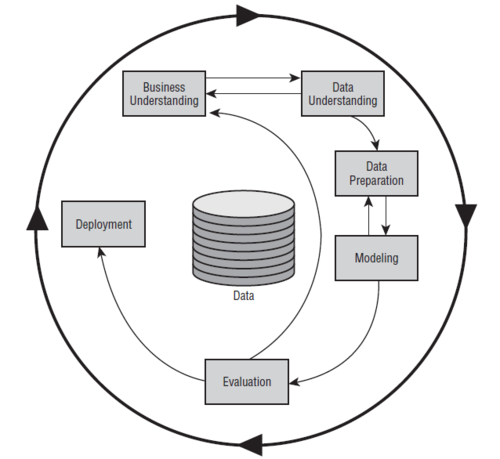
\includegraphics{https://raw.githubusercontent.com/kishkp/data621-ctg5/master/Final\%20Project/CRISP-DM.png}
\caption{CRISP-DM}
\end{figure}

\subsection{Business Understanding :}\label{business-understanding}

\subsection{Data Exploration :}\label{data-exploration-1}

5.1 Data Exploration

In section we will explore and gain some insights into the dataset by
pursuing the below high level steps and inquiries: -Variable
identification -Understanding predictor variables relationship with
response variable -Missing values and Unique Values

\subsection{Data Preparation :}\label{data-preparation-1}

\section{Methodology}\label{methodology-2}

\subsection{Business Understanding :}\label{business-understanding-1}

\subsection{Data Exploration :}\label{data-exploration-2}

5.1 Data Exploration

In section we will explore and gain some insights into the dataset by
pursuing the below high level steps and inquiries: -Variable
identification -Understanding predictor variables relationship with
response variable -Missing values and Unique Values

\subsection{Data Preparation :}\label{data-preparation-2}

\subsection{Modeling:}\label{modeling}

\subsubsection{Logistics Regression:}\label{logistics-regression}

Logistic Regression is a probabilistic statistical classification model.
It is also used to predict a binary response from a binary
predictor.Logistics model doesn't suffer a lot from severe class
imbalance. Logistic Regression creates log odds of the response as a
linear function of predictor variables. Many of the categorical
predictors in the data set for this project have sparse and unbalanced
distributions. Using logistics model with the given set of data would
need adjustment of variables to fine tune the model.

\subsubsection{Classification Tree}\label{classification-tree}

Classification Tree is used to predict the outcome of a categorical
response variable.The purpose of the analyses via tree-building
algorithms is to determine a set of logical conditional split that
permit accurate classification of cases and accurate
prediction.Effectiveness of classification tree model with binary
variable is one of the reason for selection for this analysis study.
This model though has problem with over fitting. We will also create
RandomForest model to overcome that.

\subsubsection{RandomForest Model}\label{randomforest-model}

Random Forests grows many classification trees for given set of response
and predictor variables. Each tree gives a classification, and all the
outputs from different trees are \enquote{votes} for that class. The
forest chooses the classification having the most votes (over all the
trees in the forest). Over fitting problem with the classification tree
can be overcome by this approach with weighted average of more number of
trees. This method is good for prediction but a little bit difficult to
interpret. Since we are facing the binary category,Random Forest is a
good classification method to try.

\subsection{Evaluation}\label{evaluation}

There are number of ways to evaluate the regression and classification
models based on the purpose like prediction, classification, variable
selection etc. In the given business scenario objective is to
classification of the response variable by building a model that can
predict likelihood of response from Customer. Following evaluation
criteria we have used for model evaluation:

\begin{enumerate}
\def\labelenumi{(\arabic{enumi})}
\item
  The Hosmer-Lemeshow test assesses the model calibration and how
  predicted values tend to match the predicted frequency when split by
  risk decides. This test will be used for Logistics regression model
  validation.
\item
  AUC along with Model Accuracy will be used for model evaluation.
  Accuracy is calculated based on certain threshold where as AUC is
  overall performance evaluation of model as various points.AUC criteria
  will be given more weight age for model evaluation in this case.
\end{enumerate}

\section{Experimentations:}\label{experimentations}

In this section experimentation will be carried out with the data by
formulating three different types of models with three different
approaches. Following are the three different approaches that will be
used here-

-Model 1- This model will be created by using logit function of
Generalized Logistics Model(GLM).

-Model 2: This model will be created by using Classification tree
function.

-Model 3- This model will be created by using classification technique
RandomForests model.

There are two data set given with the business case training and test
set. Training set will be used to train the model and the test set will
be used to evaluate the model performance.

\subsubsection{Logistics regression- Model
1:}\label{logistics-regression--model-1}

Logistics regression function GLM has been used to classify the campaign
response variable. Basic model generated by using GLM function has been
enhanced by making necessary adjustments to non associated predictor
variables shown as \enquote{NA} in basic model output. Next the model
has been validated by using k=5 fold cross validation press to do
necessary adjustment to the model.

\subsubsection{Interpretation from Logistics Regression
model}\label{interpretation-from-logistics-regression-model}

There were total 10 iterations been performed before final selection of
variables were made. AIC value from model 1 and model1\_update(enhanced)
model were same 13776. Hence removing variables from basic model does
not help performance wise but reduced complexity with less degrees of
freedom.By using k=5 cross validation, (\$delta) error value came out to
be low 0.06289177.

Table below provides details on significance of the variables and its
odd ratio.

\subsubsection{Classification Tree- Model
2}\label{classification-tree--model-2}

The basic idea of classification tree model is to predict a response
variable y for the campaign from predictor variables. Model does this by
growing a binary tree. At each node in the tree, a test is applied to
one of the inputs. Depending on the outcome of the test two routes to be
followed left or right. Eventually a leaf node is reached where a
prediction is made about the binary outcome of campaign response. Model
2 has been rated using the Classification function from ROCR
package.Basic model has been optimized using prune function.

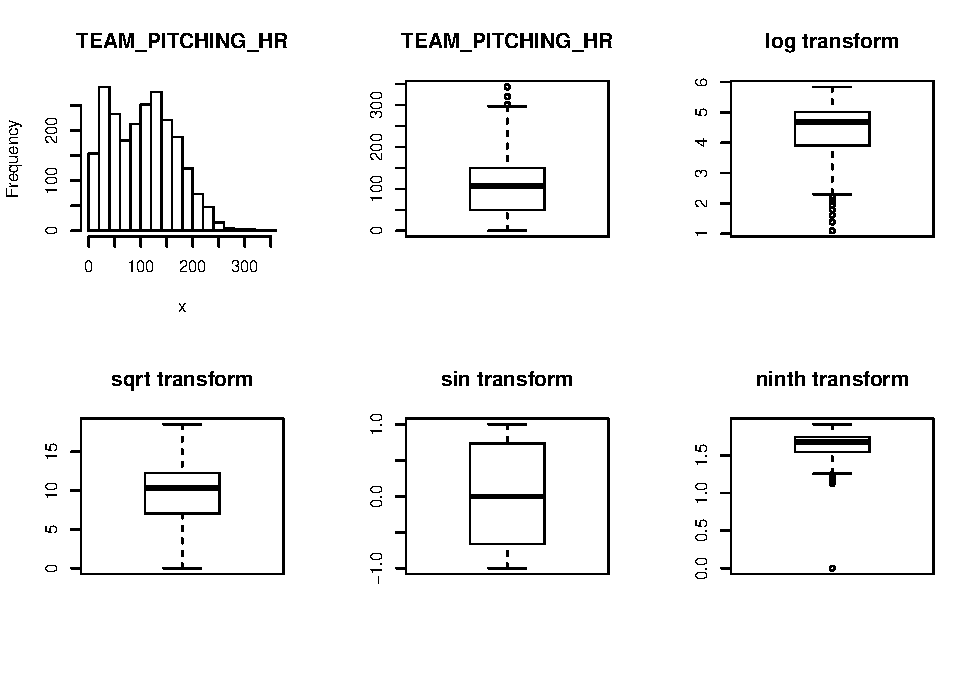
\includegraphics{apa8_files/figure-latex/unnamed-chunk-15-1.pdf}

\subsubsection{Interpretation of Classification Tree
Model}\label{interpretation-of-classification-tree-model}

Following are the most important variables from this model-duration
,nr.employed ,euribor3m ,emp.var.rate, cons.conf.idx ,
cons.price.idx.Total 6 leafs(decision points) have been formed from this
model. Complete Classification tree is given below in the diagram.

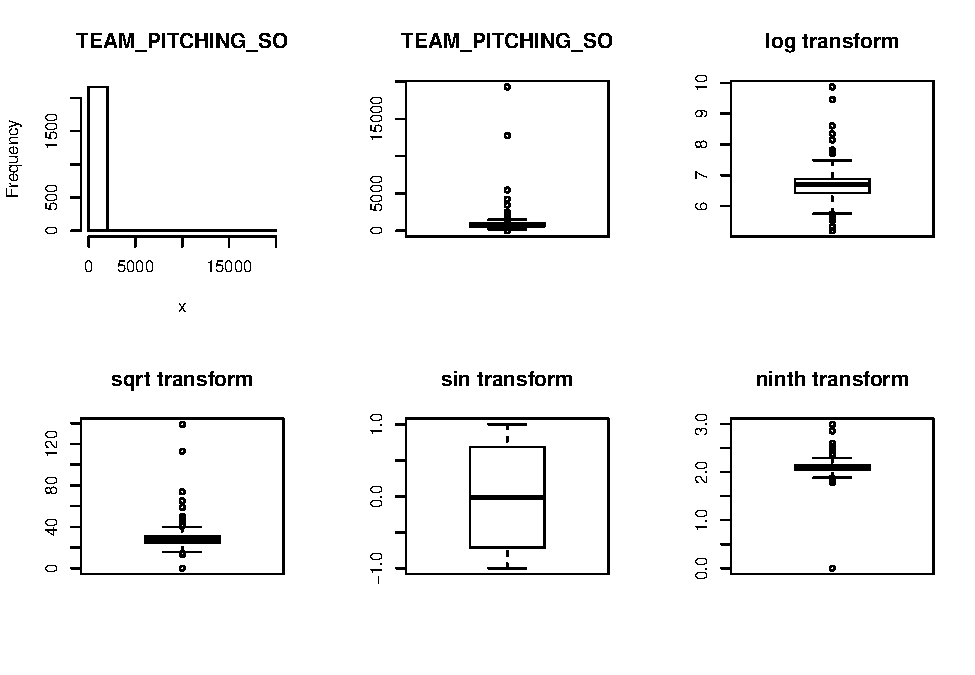
\includegraphics{apa8_files/figure-latex/unnamed-chunk-16-1.pdf}

\subsubsection{RandomForest- Model 3}\label{randomforest--model-3}

In Random Forests many classification trees are formed to classify
campaign response variable y. Each tree creates separate set of
classification, each tree is voted for performance for that
classification. The forest chooses the classification having the most
votes (over all the trees in the forest). One model will be created
using this method with tree size 50. Then this model will be evaluated
with a model of tree size 100.

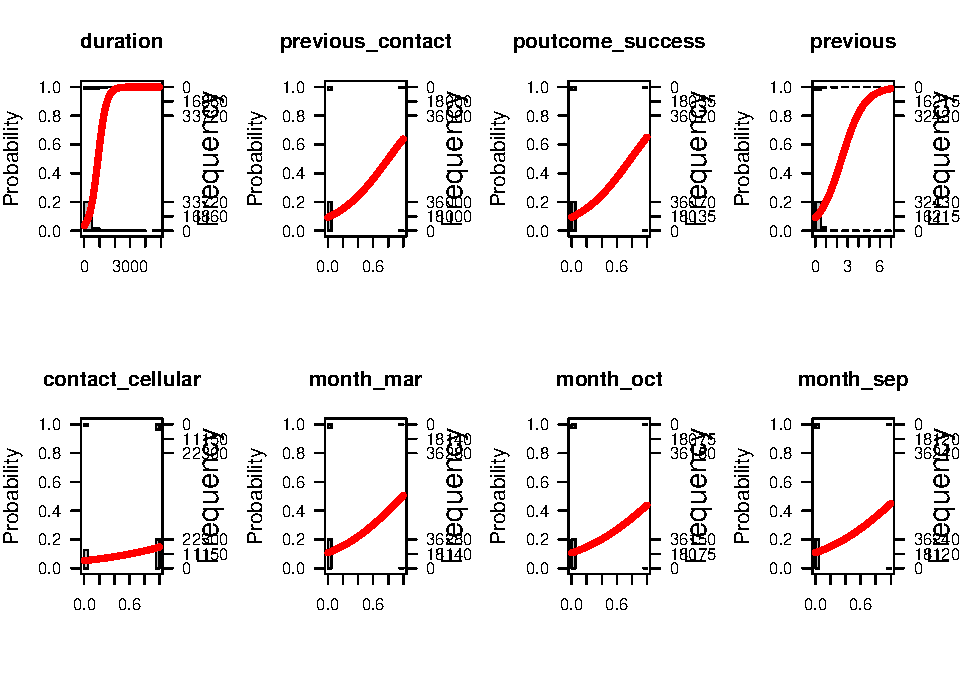
\includegraphics{apa8_files/figure-latex/unnamed-chunk-17-1.pdf}

\subsubsection{Interpretation of
RandomForest}\label{interpretation-of-randomforest}

From the chart above it can be seen that classification error rate to
classify negative responses reduces with the increase in number of trees
but there is no significant change in error rate for positive
response.There is only slight reduction in error rate for negative
responses when tree size is increased to 100 from 50.Number of variables
tried at each split are 7 with negative classification rate of 0.03 and
positive classification error rate of 0.51.

Below chart provides importance of various variables used in the model.

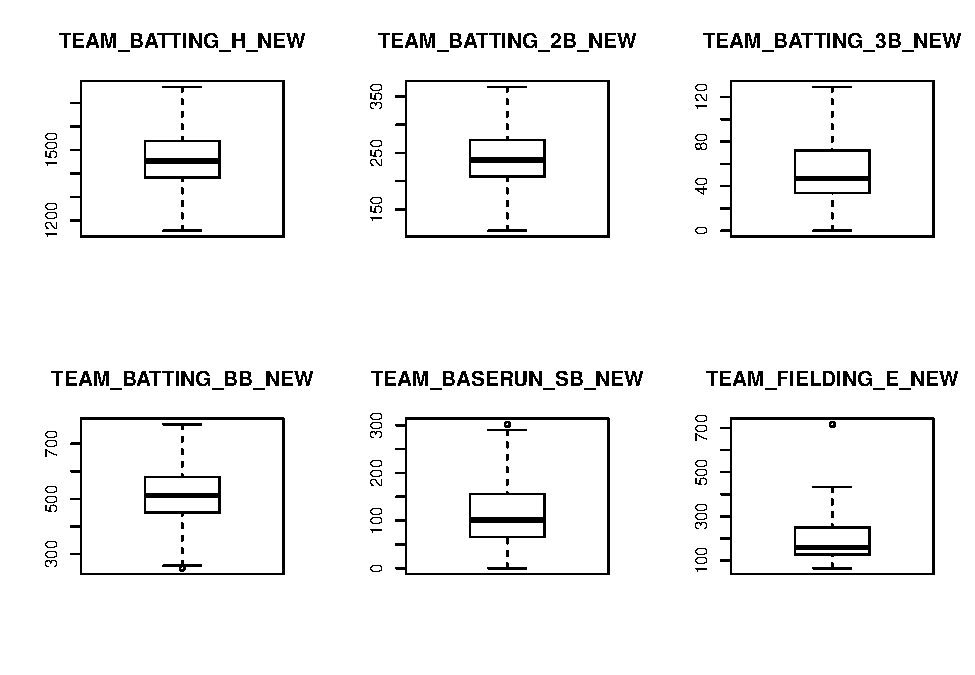
\includegraphics{apa8_files/figure-latex/unnamed-chunk-18-1.pdf}

\section{Results}\label{results}

\subsection{Results from Regression
Model}\label{results-from-regression-model}

\begin{longtable}[c]{@{}lrrrrrrr@{}}
\caption{Model 1 evaluation KPIs}\tabularnewline
\toprule
& Accuracy & Error\_Rate & Precision & sensitivity & specificity &
F1\_Score & AUC\tabularnewline
\midrule
\endfirsthead
\toprule
& Accuracy & Error\_Rate & Precision & sensitivity & specificity &
F1\_Score & AUC\tabularnewline
\midrule
\endhead
1 & 0.9142996 & 0.0857004 & 0.4323725 & 0.6678082 & 0.9331069 &
0.3607211 & 0.7029638\tabularnewline
\bottomrule
\end{longtable}

\subsection{Results from Regression
Model}\label{results-from-regression-model-1}

\begin{longtable}[c]{@{}lrrrrrrr@{}}
\caption{Model 1 evaluation KPIs}\tabularnewline
\toprule
& Accuracy & Error\_Rate & Precision & sensitivity & specificity &
F1\_Score & AUC\tabularnewline
\midrule
\endfirsthead
\toprule
& Accuracy & Error\_Rate & Precision & sensitivity & specificity &
F1\_Score & AUC\tabularnewline
\midrule
\endhead
1 & 0.9142996 & 0.0857004 & 0.4323725 & 0.6678082 & 0.9331069 &
0.3607211 & 0.7029638\tabularnewline
\bottomrule
\end{longtable}

From above table it can be seen Logistics Regression model has a very
high accuracy rate of 91.42\% when model was evaluated using the
validation data set. Though the AUC value for this model was
comparatively lower 0.702 which indicates not good fitment of the model.

\begin{verbatim}
Hosmer and Lemeshow goodness of fit (GOF) test
\end{verbatim}

data: model1\_update\$y, fitted(m) X-squared = 14.926, df = 8, p-value =
0.0606

By using Hosmer-Lemeshow goodness-of-fit (GOF) tests when model was
evaluated p value came to be greater than 0.05. With this test if the p
value is lower than 0.05 model is rejected and if it's high, then the
model passes the test. Regression model passed this test.

\subsection{Results from Classification Tree- Model
2}\label{results-from-classification-tree--model-2}

\begin{longtable}[c]{@{}lrrrrrrr@{}}
\caption{Model 1 evaluation KPIs}\tabularnewline
\toprule
& Accuracy & Error\_Rate & Precision & sensitivity & specificity &
F1\_Score & AUC\tabularnewline
\midrule
\endfirsthead
\toprule
& Accuracy & Error\_Rate & Precision & sensitivity & specificity &
F1\_Score & AUC\tabularnewline
\midrule
\endhead
2 & 0.918184 & 0.081816 & 0.5343681 & 0.6548913 & 0.9440149 & 0.4377405
& 0.8650875\tabularnewline
\bottomrule
\end{longtable}

It can be seen from the table above, this model 2 has also very high
accuracy rate of 91.81\% which is very good.This model has AUC value of
0.865 which seem to be inline with given high accuracy.

\subsection{Results from RandomForest
Model}\label{results-from-randomforest-model}

\begin{longtable}[c]{@{}lrrrrrrr@{}}
\caption{Model 1 evaluation KPIs}\tabularnewline
\toprule
& Accuracy & Error\_Rate & Precision & sensitivity & specificity &
F1\_Score & AUC\tabularnewline
\midrule
\endfirsthead
\toprule
& Accuracy & Error\_Rate & Precision & sensitivity & specificity &
F1\_Score & AUC\tabularnewline
\midrule
\endhead
3 & 0.9752367 & 0.0247633 & 0.8115299 & 0.9556136 & 0.9772484 &
0.8024464 & 0.9034476\tabularnewline
\bottomrule
\end{longtable}

The model created using Randomforest has accuracy of 98.64\% which is
extraordinary results and give rise to suspicion model is able to
separate out the classification based on certain variable. When we
looked at the importance of variable \enquote{duration} it becomes
apparent that this variable is being used in a big way to classify
response accurately. It can be seen that this model also shows the
similar kind of trend in classification of data in earlier stages with
very stiff line till true positive rate of 0.4 and then sharp increase
in false positive rate.

\section{5 Discussion and
Conclusions:}\label{discussion-and-conclusions}

\begin{longtable}[c]{@{}llrrrrrrr@{}}
\caption{Comparison of 3 Model3}\tabularnewline
\toprule
& Model\_No & Accuracy & Error\_Rate & Precision & sensitivity &
specificity & F1\_Score & AUC\tabularnewline
\midrule
\endfirsthead
\toprule
& Model\_No & Accuracy & Error\_Rate & Precision & sensitivity &
specificity & F1\_Score & AUC\tabularnewline
\midrule
\endhead
1 & GLM\_model1 & 0.9142996 & 0.0857004 & 0.4323725 & 0.6678082 &
0.9331069 & 0.3607211 & 0.7029638\tabularnewline
2 & CRT\_model2 & 0.9181840 & 0.0818160 & 0.5343681 & 0.6548913 &
0.9440149 & 0.4377405 & 0.8650875\tabularnewline
3 & RF\_model3 & 0.9752367 & 0.0247633 & 0.8115299 & 0.9556136 &
0.9772484 & 0.8024464 & 0.9034476\tabularnewline
\bottomrule
\end{longtable}

\includegraphics{apa8_files/figure-latex/unnamed-chunk-25-1.pdf}

\$ Final model selection:

Based on the Accuracy of the model, model 1 and model 2 are very close
around 91\% accuracy with probability threshold of 0.5. Model 3 has much
higher value of 98\%. But Accuracy is not always the key criteria for a
model as Accuracy is calculated based on a defined threshold. Also due
to imbalance of data o 10\% to 90\% distribution of response variable
forced to choose the model based on other criteria. Model Based on AUC
value is model 3 having AUC value of 0.9398 which is a very good score.
Model 3 stands out among the three models.

\$ Key predictor variables:

For all three models it is found variables \enquote{duration} is most
important variables by far. This variable has positive impact in
campaign outcome. This could be due to the fact that longer the Customer
stays on phone more productive conversation is taking place to get the
Customer start their term deposit Account. \enquote{euribor3m} is most
important variable which denotes inter bank interest rate in Eurozone.
Term deposit interest rates are generally interlinked and tends to go up
together. This variable has positive impact on response variable.
Predictor \enquote{nr.employed} denotes number of employees for the
bank. This variable also has positive impact on campaign response. More
the number of employees more visible the bank is and in turn more
customers it gets through the campaign.

Among the negative variables \enquote{emp.var.rate} has negative impact
on response. As negative rate of this variable indicates issues with
economy and lower economic activities. That in turn could impact the
savings rate and people tend to use their savings that time.

\$ Shortcomings

Imbalance of response variable only 10\% of population was the main
shortcomings that we have in the model creation. This issue has been
addressed partially by using Area Under Curve as the criteria for model
selection.

\$ Final Recommendation

In conclusion it can be suggested to the bank management that focus
should be given in hiring more people, doing more quality phone calls.
Also to time the campaign in a stable macroeconomic environment to get
better return on investment from this campaign.

\section{References}\label{references}

be sure to cite all references used in the report (APA format). We used
R (3.2.3, R Core Team, 2016) and the R-packages \emph{papaja}
(0.1.0.9054, Aust \& Barth, 2015), and \emph{papaja} (0.1.0.9054, Aust
\& Barth, 2015) for all our analyses.

\section{Appendix}\label{appendix}

Supplemental tables and/or figures. R statistical programming code.

\section{\texttt{\{r code=readLines(knitr::purl(\textquotesingle{}https://raw.githubusercontent.com/kishkp/data621-ctg5/master/HW4/HW04\_Group5.Rmd\textquotesingle{}, documentation = 0)), eval = FALSE\} \#}}\label{r-codereadlinesknitrpurlhttpsraw.githubusercontent.comkishkpdata621-ctg5masterhw4hw04ux5fgroup5.rmd-documentation-0-eval-false}

\section{6.1 Data Analysis details}\label{data-analysis-details}

\subsection{6.1.1 Variable Description}\label{variable-description}

\begin{longtable}[c]{@{}llll@{}}
\caption{Variable Description}\tabularnewline
\toprule
Variable & Data.Type & Type & Description\tabularnewline
\midrule
\endfirsthead
\toprule
Variable & Data.Type & Type & Description\tabularnewline
\midrule
\endhead
age & Numeric & Predictor & Client's age\tabularnewline
job & Catagorical & Predictor & Client's job\tabularnewline
marital & Catagorical & Predictor & Client's marital
status\tabularnewline
education & Catagorical & Predictor & Client's education
level\tabularnewline
default & Binary & Predictor & Credit in default?\tabularnewline
balance & Numeric & Predictor & Client's average yearly balance, in
euros\tabularnewline
housing & Binary & Predictor & Client has housing loan?\tabularnewline
loan & Binary & Predictor & Client has personal loan?\tabularnewline
contact & Catagorical & Predictor & Client's contact communication
type\tabularnewline
day & Catagorical & Predictor & Client last contact day of the
month\tabularnewline
month & Catagorical & Predictor & Client last contact month of
year\tabularnewline
duration & Numeric & Predictor & Client last contact duration, in
seconds\tabularnewline
campaign & Numeric & Predictor & Client number of contacts performed
during this campaign\tabularnewline
pdays & Numeric & Predictor & Client days that passed after first
contact\tabularnewline
previous & Numeric & Predictor & Number of contacts performed before
this campaign\tabularnewline
poutcome & Catagorical & Predictor & Outcome of the previous marketing
campaign\tabularnewline
emp.var.rate & Numeric & Predictor & Quarterly employment variation
rate\tabularnewline
cons.price.idx & Numeric & Predictor & Monthly consumer price
index\tabularnewline
cons.conf.idx & Numeric & Predictor & Monthly consumer confidence
index\tabularnewline
euribor3m & Numeric & Predictor & Daily euribor 3 month
rate\tabularnewline
nr.employed & Numeric & Predictor & Quarterly number of
employees\tabularnewline
y & Binary & Response & Has the client subscribed a term
deposit?\tabularnewline
\bottomrule
\end{longtable}

\subsection{6.1.2 Predictor and Response variable
Association}\label{predictor-and-response-variable-association}

\includegraphics{apa8_files/figure-latex/unnamed-chunk-27-1.pdf}
\includegraphics{apa8_files/figure-latex/unnamed-chunk-27-2.pdf}
\includegraphics{apa8_files/figure-latex/unnamed-chunk-27-3.pdf}
\includegraphics{apa8_files/figure-latex/unnamed-chunk-27-4.pdf}
\includegraphics{apa8_files/figure-latex/unnamed-chunk-27-5.pdf}
\includegraphics{apa8_files/figure-latex/unnamed-chunk-27-6.pdf}
\includegraphics{apa8_files/figure-latex/unnamed-chunk-27-7.pdf}
\includegraphics{apa8_files/figure-latex/unnamed-chunk-27-8.pdf}
\includegraphics{apa8_files/figure-latex/unnamed-chunk-27-9.pdf}
\includegraphics{apa8_files/figure-latex/unnamed-chunk-27-10.pdf}
\includegraphics{apa8_files/figure-latex/unnamed-chunk-27-11.pdf}
\includegraphics{apa8_files/figure-latex/unnamed-chunk-27-12.pdf}
\includegraphics{apa8_files/figure-latex/unnamed-chunk-27-13.pdf}
\includegraphics{apa8_files/figure-latex/unnamed-chunk-27-14.pdf}
\includegraphics{apa8_files/figure-latex/unnamed-chunk-27-15.pdf}
\includegraphics{apa8_files/figure-latex/unnamed-chunk-27-16.pdf}
\includegraphics{apa8_files/figure-latex/unnamed-chunk-27-17.pdf}
\includegraphics{apa8_files/figure-latex/unnamed-chunk-27-18.pdf}
\includegraphics{apa8_files/figure-latex/unnamed-chunk-27-19.pdf}
\includegraphics{apa8_files/figure-latex/unnamed-chunk-27-20.pdf}

\subsection{6.1.3 Unique Value \& Missing
value}\label{unique-value-missing-value}

We see that there are no missing values in our dataset as shown in table
2 and graph format. The unique values are given in the table

\begin{longtable}[c]{@{}lr@{}}
\caption{Missing Values}\tabularnewline
\toprule
& Missing Values\tabularnewline
\midrule
\endfirsthead
\toprule
& Missing Values\tabularnewline
\midrule
\endhead
age & 0\tabularnewline
job & 0\tabularnewline
marital & 0\tabularnewline
education & 0\tabularnewline
default & 0\tabularnewline
housing & 0\tabularnewline
loan & 0\tabularnewline
contact & 0\tabularnewline
month & 0\tabularnewline
day\_of\_week & 0\tabularnewline
duration & 0\tabularnewline
campaign & 0\tabularnewline
pdays & 0\tabularnewline
previous & 0\tabularnewline
poutcome & 0\tabularnewline
emp.var.rate & 0\tabularnewline
cons.price.idx & 0\tabularnewline
cons.conf.idx & 0\tabularnewline
euribor3m & 0\tabularnewline
nr.employed & 0\tabularnewline
y & 0\tabularnewline
\bottomrule
\end{longtable}

\begin{longtable}[c]{@{}lr@{}}
\caption{Unique Values}\tabularnewline
\toprule
& Unique Values\tabularnewline
\midrule
\endfirsthead
\toprule
& Unique Values\tabularnewline
\midrule
\endhead
age & 78\tabularnewline
job & 12\tabularnewline
marital & 4\tabularnewline
education & 8\tabularnewline
default & 3\tabularnewline
housing & 3\tabularnewline
loan & 3\tabularnewline
contact & 2\tabularnewline
month & 10\tabularnewline
day\_of\_week & 5\tabularnewline
duration & 1544\tabularnewline
campaign & 42\tabularnewline
pdays & 27\tabularnewline
previous & 8\tabularnewline
poutcome & 3\tabularnewline
emp.var.rate & 10\tabularnewline
cons.price.idx & 26\tabularnewline
cons.conf.idx & 26\tabularnewline
euribor3m & 316\tabularnewline
nr.employed & 11\tabularnewline
y & 2\tabularnewline
\bottomrule
\end{longtable}

\subsection{6.1.4 Data Summary post
conversion}\label{data-summary-post-conversion}

\subsection{6.1.5 Outliers Analysis}\label{outliers-analysis}

\includegraphics{apa8_files/figure-latex/unnamed-chunk-30-1.pdf}

\subsection{6.1.6 Analysis of link functions for given
variables}\label{analysis-of-link-functions-for-given-variables}

\setlength{\parindent}{-0.5in} \setlength{\leftskip}{0.5in}
\setlength{\parskip}{11pt}

Aust, F., \& Barth, M. (2015). \emph{Papaja: Create aPA manuscripts with
rMarkdown}. Retrieved from \url{https://github.com/crsh/papaja}

R Core Team. (2016). \emph{R: A language and environment for statistical
computing}. Vienna, Austria: R Foundation for Statistical Computing.
Retrieved from \url{https://www.R-project.org/}



\end{document}
